\begin{frame}{Uncertainty }
\begin{columns}

\column{.25\textwidth}
\begin{figure}[ht]
\includegraphics[width=\textwidth]{images/wind}
\end{figure}
Windspeed \\30 km/hr
\pause
\column{.25\textwidth}
\begin{figure}[ht]
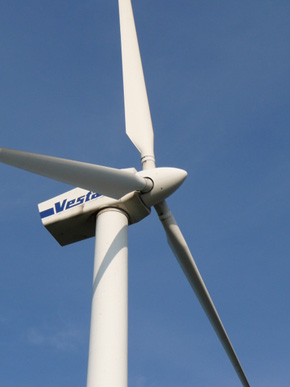
\includegraphics[width=\textwidth]{images/windmill}
\end{figure}
Wind Power \\ 50 KW

\pause
\column{.25\textwidth}
\begin{figure}[ht]
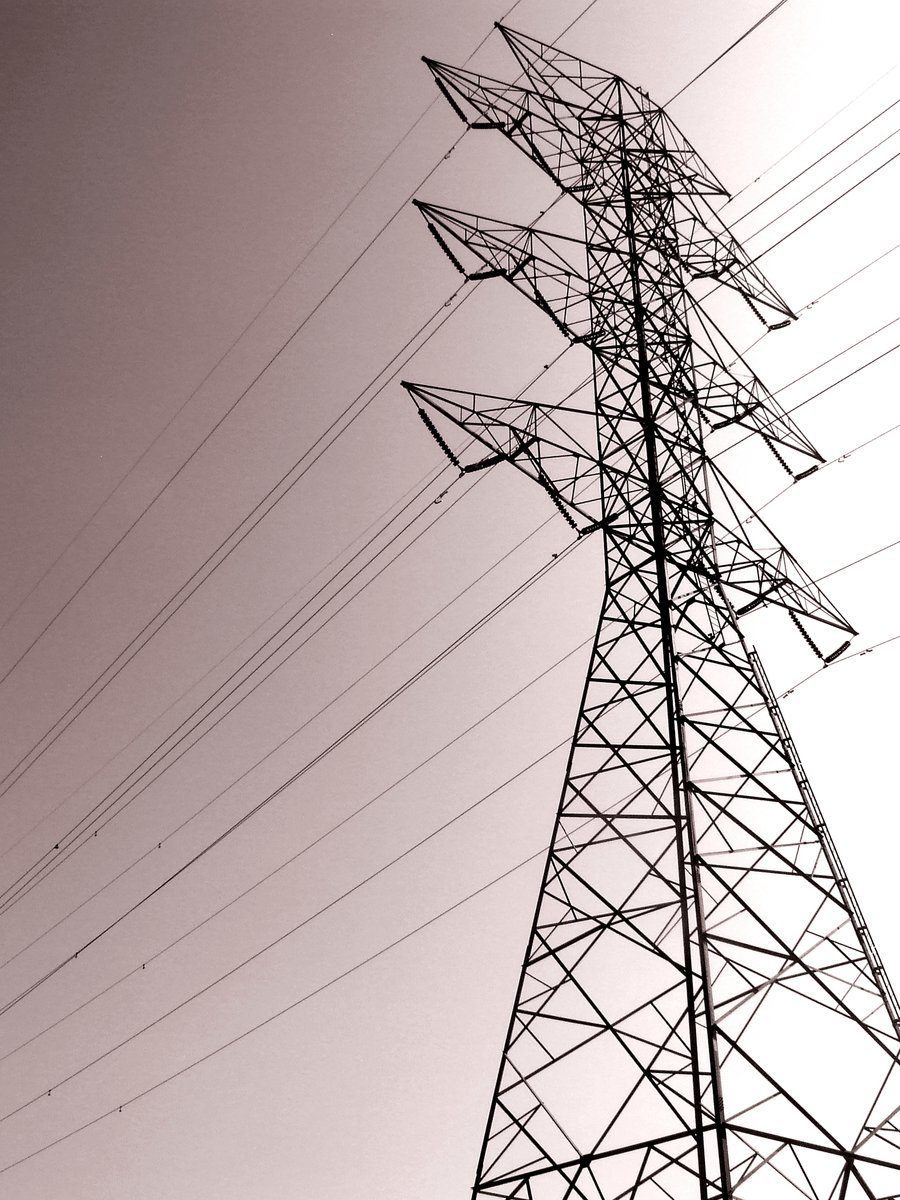
\includegraphics[width=\textwidth]{images/electricity}
\end{figure}
Electricity \\ 40 KW

\pause
\column{.25\textwidth}
\begin{figure}[ht]
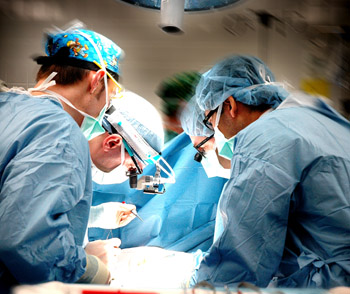
\includegraphics[width=\textwidth]{images/surgery}
\end{figure}
Lights are on!

\end{columns}
\end{frame}


\begin{frame}{Uncertainty }
Measurements are Distributions, not Scalars

\begin{columns}

\column{.25\textwidth}
\begin{figure}[ht]
\includegraphics[width=\textwidth]{images/wind}
\end{figure}
WindSpeed:
Around 30 km/hr
\begin{figure}[ht]
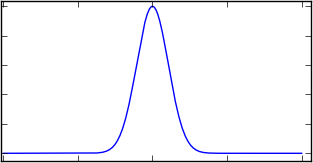
\includegraphics[width=\textwidth]{images/normal}
\end{figure}

\column{.25\textwidth}
\begin{figure}[ht]
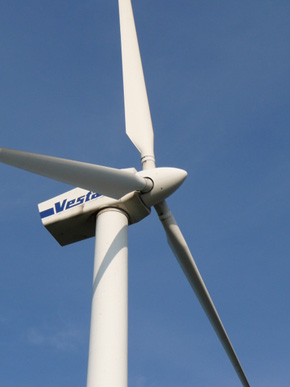
\includegraphics[width=\textwidth]{images/windmill}
\end{figure}
WindPower:
\begin{figure}[ht]
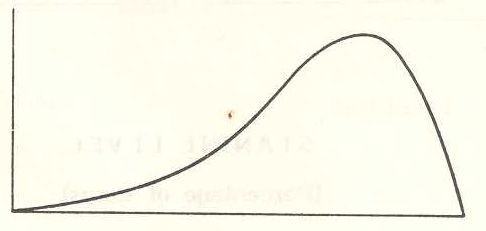
\includegraphics[width=\textwidth]{images/skew}
\end{figure}

\column{.25\textwidth}
\begin{figure}[ht]
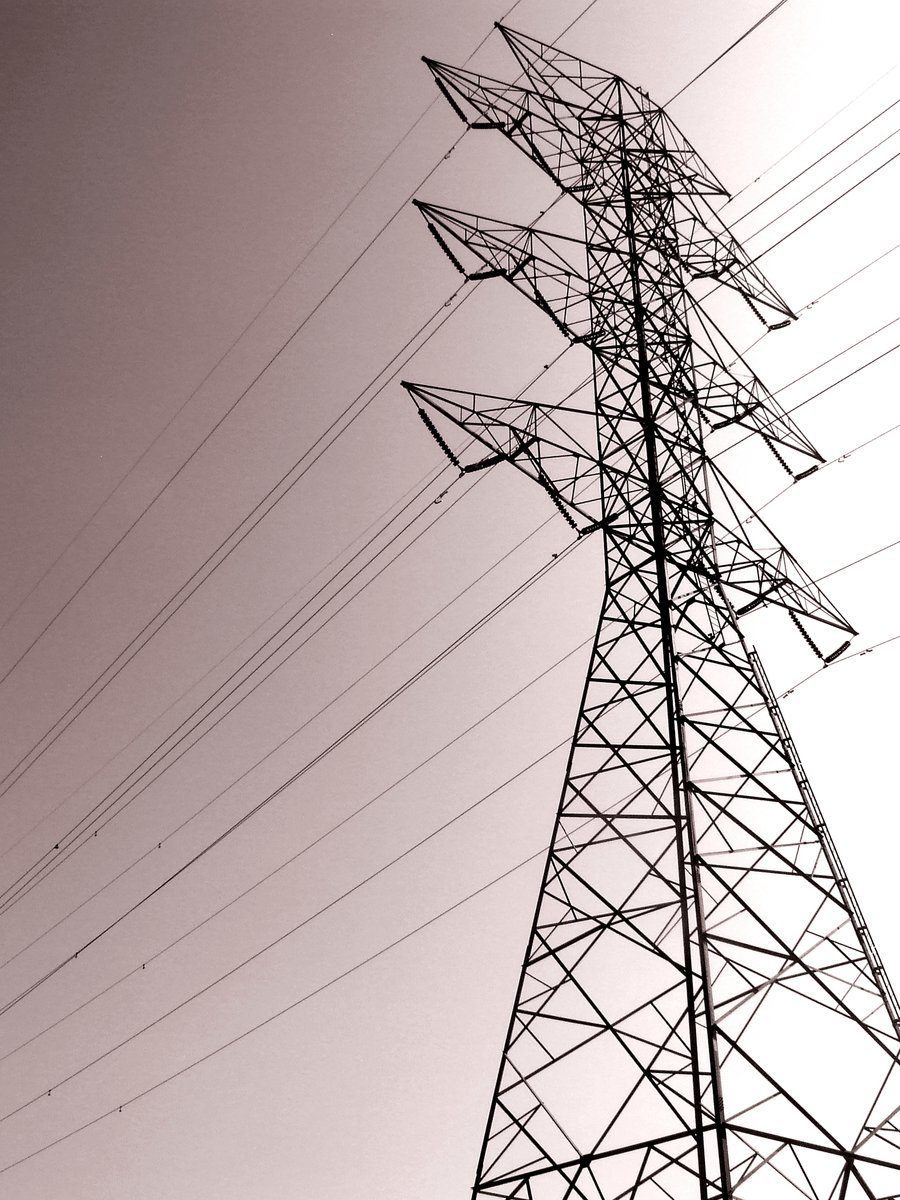
\includegraphics[width=\textwidth]{images/electricity}
\end{figure}
Electricity:
\begin{figure}[ht]
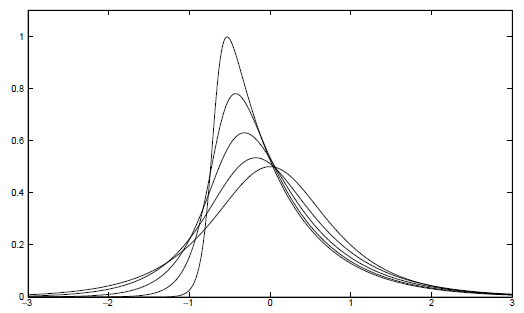
\includegraphics[width=\textwidth]{images/skew2}
\end{figure}

\column{.25\textwidth}
\begin{figure}[ht]
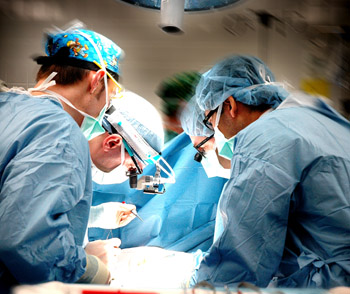
\includegraphics[width=\textwidth]{images/surgery}
\end{figure}
Lights stay on?

\end{columns}

\end{frame}
